%%____________________________________________________________________________||
\section{Trigger strategy}
\label{sec:triggers}


\subsection{Hadronic signal region\label{sec:hadronic_signal_region}}

In Run~2 the RA1 analysis retains the low-thresholds of Run~1 with developments 
to the trigger selection, maintaining sensitivity to signatures of new physics with hadronic 
energies as low as $\scalht = 200$ GeV. This in part is achieved by a migration to PF-based 
jet reconstruction within the HLT which, in conjunction with a reduction of clustering radius 
parameter $\Delta R = 0.4$, provides improvements in jet energy resolution in high-pileup 
conditions and mitigates the effects of pileup contamination within the jet cone.

The RA1 analysis utilises a range of triggers for the selection of events in the hadronic signal region
to provide coverage over a wide range of event topologies. A guiding principle of the analysis is to be as
inclusive as possible by probing low thresholds, necessitating operation in or near the trigger turn-on.

Events in the hadronic monojet signal region are selected with the use of a single \mht-\met cross-trigger, 
\verb!HLT_PFMETNoMu90_JetIdCleaned_PFMHTNoMu90_IDTight!, which is cross-cleaned of muons in the computation 
of event variables in the HLT. 

A suite of $\scalht$-$\alphat$ cross-triggers 
with a requirement on the average \pt of the leading two jets, $\pt^{\rm \left<j1,j2\right>}$, 
are utilised in the selection of events in the hadronic multijet signal region, labelled: 
\verb!HLT_PFHTXXX_PFDijetYYY_AlphaT0pZZ!. The use of a dijet average threshold provides an improved 
suppression of QCD multijet events within the trigger,
enabling looser \alphat thresholds to be utilised whilst maintaining acceptance to events exhibiting asymmetric jet 
topologies such as monojet-like signatures of compressed spectrum and DM models. It was found that a dijet average
threshold of 90 \GeV ensured the optimum performance when balancing efficiency and rate, with both the $\scalht$ and $\alphat$
thresholds across all jet toplogies. The dijet average requirement does however lead to a loss in efficiency for 
asymmetric jet events where the sub-leading jet is soft. This loss in efficiency is mitigated by taking the 
disjunction of the \verb!HLT_PFHTXXX_PFDijetYYY_AlphaT0pZZ! and the monojet triggers which provides a recovery 
of efficiency in the turn-on and close to the plateau. The $\scalht$-$\alphat$ triggers seed all signal multijet offline 
bins in the range for $\scalht > 200$ \GeV. Above $\scalht > 800$ an additional pure \scalht trigger, \verb!HLT_PFHT800!, 
is utilised which has no explicit dependence on $\alphat$ or dijet average threshold. 

These triggers form the primary signal selection menu for the analysis, in addition a set of secondary triggers with 
higher thresholds were in operation to provide redundancy for higher luminosity scenarios. In Run 2 however the primary 
triggers sufficiently suppressed trigger rates such that the use of secondary triggers in the analysis are not required.


The Level-1 seeds for the $\scalht$-$\alphat$ HLT paths are given by the disjunction of the lowest 
unprescaled Level-1 hadronic scalar energy and missing energy sum seeds (\verb!HTTXXX_OR_ETMYYY!) for 
the given run scenario. A loose calorimeter trigger prefilter is utilised to reduce the pass-through 
rate prior to track-based reconstruction, ensuring the PF-based filters meet timing requirements. The calorimeter prefilter 
utilises loose \scalht and dijet average \pt requirements in addition to a new variable \alphat', 
defined as \alphat in the limit $\Delta\scalht \rightarrow 0$, which better correlates \alphat 
between calorimeter and PF-based reconstruction. The monojet and \verb!HLT_HT800! triggers use the
\verb!ETMYYY!

The thresholds of the signal triggers are shown in Table~\ref{tab:2015_Hadronic_Signal_Triggers}. The choice of threshold for 
the \scalht-\alphat triggers were tuned to maintain acceptance for a range of signal topologies whilst effectively suppressing QCD 
multijet events to maintain acceptable trigger rates. 




% TABLE : 2015 triggers
%----------------------------------------------------------------------
\begin{table}[h!]
\topcaption{Trigger thresholds of the Level-1, calorimeter prefilter and final PF-trigger decision for
 the primary HLT paths for the hadronic signal region in the $\lumi=7\times10^{33}\cm^{-2}{\rm s}^{-1}$ scenario.
 Higher threshold Level-1 \scalht and \met seeds are utilised for the higher luminosity scenario. }
\footnotesize
\centering
\begin{tabular}{c|cccc} 
\hline
\hline
HLT path     & L1 seed & HLT calo-prefilter & HLT PF-filter                                                \\
    &        & ($\scalht$, $\alphat$', $\pt^{\rm \left<j1,j2\right>}$, \met) & ($\scalht$, $\alphat$, $\pt^{\rm \left<j1,j2\right>}$, \met) \\ %& (Hz) \\[0.7 ex] 
\hline
{\scriptsize \verb!HLT_PFHT200_PFDijetAve90_AlphaT0p57!} & {\scriptsize \verb!HTT125 OR ETM50!} & 150, 0.540, 70, - & 200, 0.570, 90, - \\ %& \\ % 11.0 $\pm$ 3.0 \\
{\scriptsize \verb!HLT_PFHT250_PFDijetAve90_AlphaT0p55!} & {\scriptsize \verb!HTT125 OR ETM50!} & 200, 0.535, 70, - & 250, 0.550, 90, - \\ %& \\ % 8.5  $\pm$ 3.0 \\
{\scriptsize \verb!HLT_PFHT300_PFDijetAve90_AlphaT0p53!} & {\scriptsize \verb!HTT125 OR ETM50!} & 250, 0.525, 70, - & 300, 0.530, 90, - \\ %& \\ % 9.5  $\pm$ 3.0 \\
{\scriptsize \verb!HLT_PFHT350_PFDijetAve90_AlphaT0p52!} & {\scriptsize \verb!HTT125 OR ETM50!} & 300, 0.520, 70, - & 350, 0.520, 90, - \\ %& \\ % 10.0 $\pm$ 3.0 \\
{\scriptsize \verb!HLT_PFHT400_PFDijetAve90_AlphaT0p51!} & {\scriptsize \verb!HTT125 OR ETM50!} & 370, 0.510, 70, - & 400, 0.510, 90, - \\ %& \\ % 13.5 $\pm$ 3.5 \\ \\ %\hline \\ %
{\scriptsize \verb!HLT_PFHT800!}                         & {\scriptsize \verb!HTT175!}          & 650, -, -, -      & 800, -, -, -, -   \\ %& \\ % 13.5 $\pm$ 3.5 \\ \\ %\hline \\ %
{\scriptsize \verb!HLT_PFMETNoMu90_PFMHTNoMu90_IDTight!} & {\scriptsize \verb!ETM50!}           &  -, -, -, -, 65   & -, -, -, -, 90    \\
%% L1sL1ETM70ORETM60ORETM50
%% hltMET, MHT 65
\hline
\hline
\end{tabular}
\label{tab:2015_Hadronic_Signal_Triggers}
\end{table}


An important goal of the analysis is to have good acceptance
to compressed SUSY and general DM models. It is therefore critical
that we operate in the trigger turn on regions for the lower
thresholds. We have already successfully exercised this approach with 
the Run 1 analysis and will repeat this mode or operating during Run 2.
As in Run~1, multiple efficiency measurements are
employed, which are performed with data and propagated through to the
analysis with cross checks in simulation. A summary of estimates of a 
selection of signal models in simulation is presented in Appendix~\ref{app:signalModelTriggerEfficiencies}.

%% However, it is noted that for the majority of models accessible by the
%% "Early Analysis", such as gluino-induced production and decay, the
%% most sensitive bins are typically at higher values of MHT, for which
%% the triggers perform close to full efficiency. Lower MHT bins are
%% subject to trigger efficiency corrections based on measurements in
%% data, as discussed above. 


% 

The efficiency of the signal triggers are measured in data using electron and muon samples 
selected by the unprescaled \verb!HLT_Ele23_eta2p1_WPLoose_Gsf! and \verb!HLT_IsoMu20! 
reference triggers with a signal selection. Biases in these measurements can be introduced 
due to the contamination in the computation of event variables and different treatments 
between trigger and offline reconstructions, the degree of which varies with \scalht and \njet.

The monojet trigger performs a cross-cleaning of muons online, enabling its efficiency to measured
in an unbiased manner using a muon sample. Electrons however cannot be disentangled and to remain 
consisent with the trigger must be measured with offline cross-cleaning disabled. A comparison of 
the estimate of the monojet trigger efficiency using muon and electron samples is shown in Fig.~\ref{fig:gjets_HTsideband}.


Compare monojet muon and electron (turnons) 


state bias in electron sample has decreasing importance for increasing HT, NJet. 
Our belief is that the proper treatment of cross-cleaning online with a muon sample (as shown in the monojet case) would produvde faster
turn ons, however the multijet triggers do not have the muon cross-cleaning. 




The trigger efficiency measurement of the multijet signal triggers in data are primarily performed with the use of 
an electron sample, selected by the unprescaled \verb!HLT_Ele23_eta2p1_WPLoose_Gsf! reference trigger with a cross. 
To remain consistent with the reconstruction of electrons in the trigger, no cross-cleaning of electrons from jets 
are performed offline, with the electron being included in the computation of event-level jet energy sums, such as 
\scalht, \MHT and \alt. 

The \verb!HLT_PFHT800! 
trigger, used to seed the analysis bin $\scalht > 800$ GeV, 
has no \alt requirement and thus no \alt turn-on is shown for this path.

{
The trigger efficiency estimates with the electron reference trigger are found to be close to or at the plateau when taking the disjunction of the 
triggers for \scalht < 800 \GeV. Full efficiency is therefore assume for these triggers with a systematic to this estimate assigned equal to the 
inefficiency estimated by the respective reference trigger. For \scalht > 800 \GeV, where the bias of electrons is a smaller effect, the trigger 
efficiency is measured for the disjunction of the \scalht-\alphat and \verb!HLT_HT800! triggers, inclusively on jet multiplicity, and a correction applied. 


Turn-on for the individual triggers \alphat Appendix~\ref{app:alphaTTriggerEfficiencies}
}



\begin{figure}[h!]
  \begin{center}
    \subfigure[\njet = 1]{\includegraphics[width=0.5\textwidth]{figures/Trigger/HLT_IsoMu20/HLT_PFMETNoMu90_JetIdCleaned_PFMHTNoMu90_IDTight_MoM_Mono_MHT0_ht_Fit}} ~~ 
    \caption{
          }
    \label{fig:alphat_turnons}
  \end{center} 
\end{figure}


\begin{figure}[h!]
  \begin{center}
    \subfigure[$200 < \scalht < 250$]{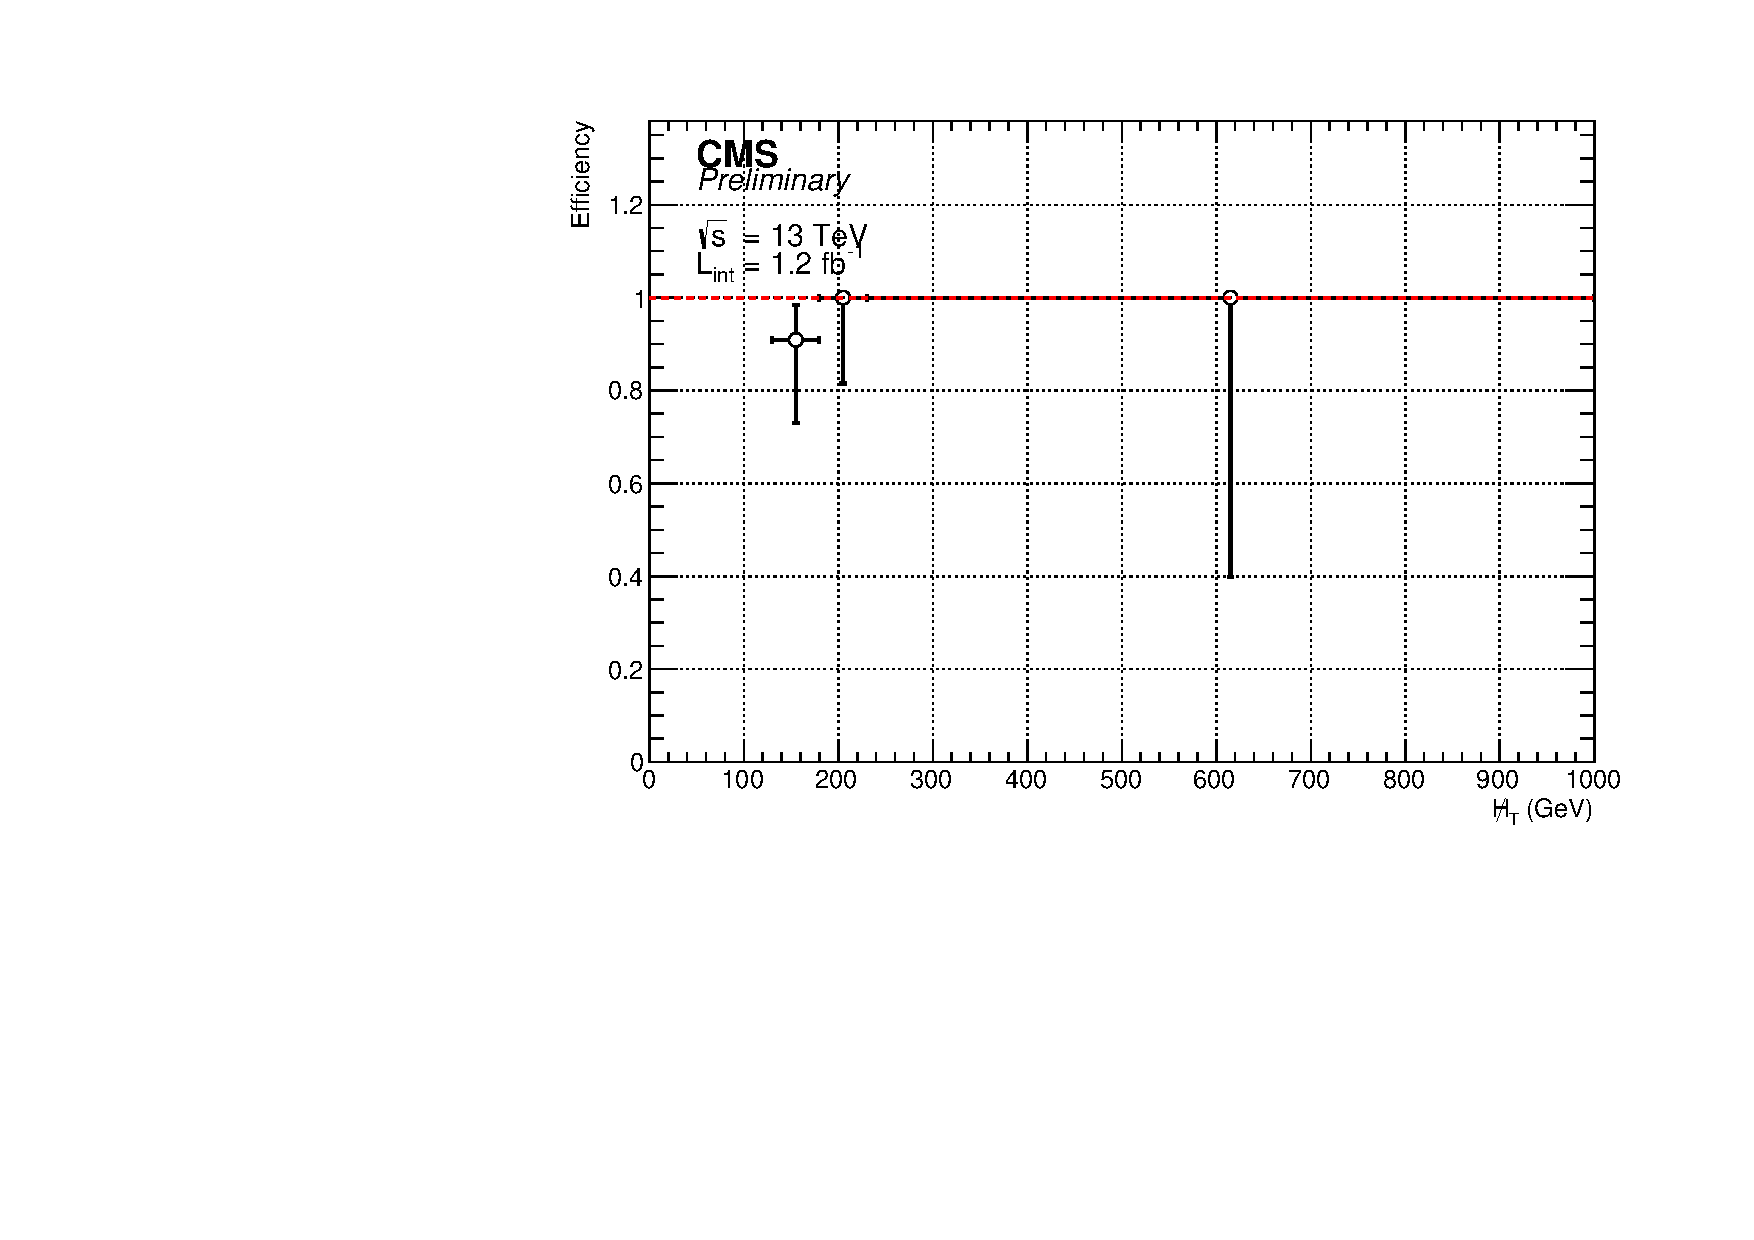
\includegraphics[width=0.5\textwidth]{figures/Trigger/HLT_Ele23_eta2p1_WPLoose_Gsf/HLT_AlphaTMonoAll_MoM_200to250_mht}} ~~\
    \subfigure[$250 < \scalht < 300$]{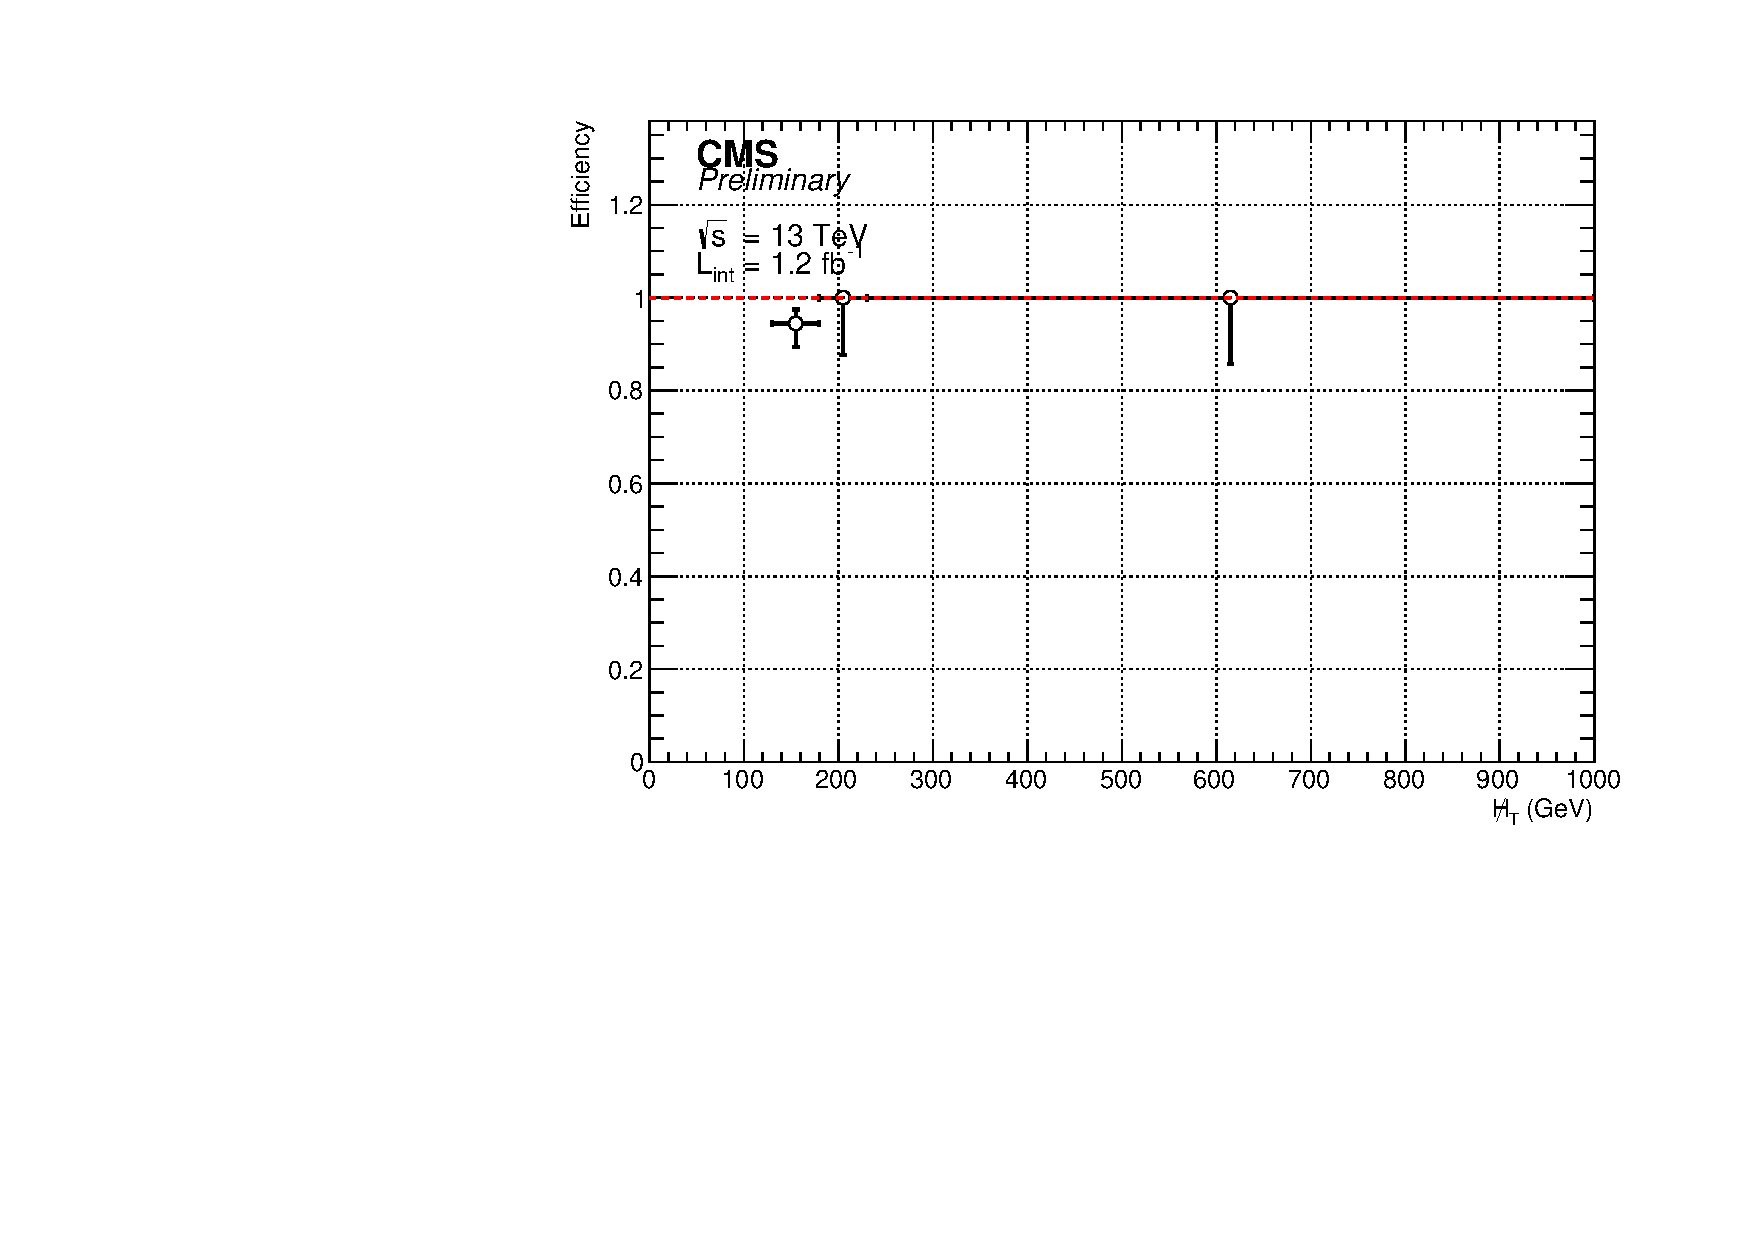
\includegraphics[width=0.5\textwidth]{figures/Trigger/HLT_Ele23_eta2p1_WPLoose_Gsf/HLT_AlphaTMonoAll_MoM_250to300_mht}} \\
    \subfigure[$300 < \scalht < 350$]{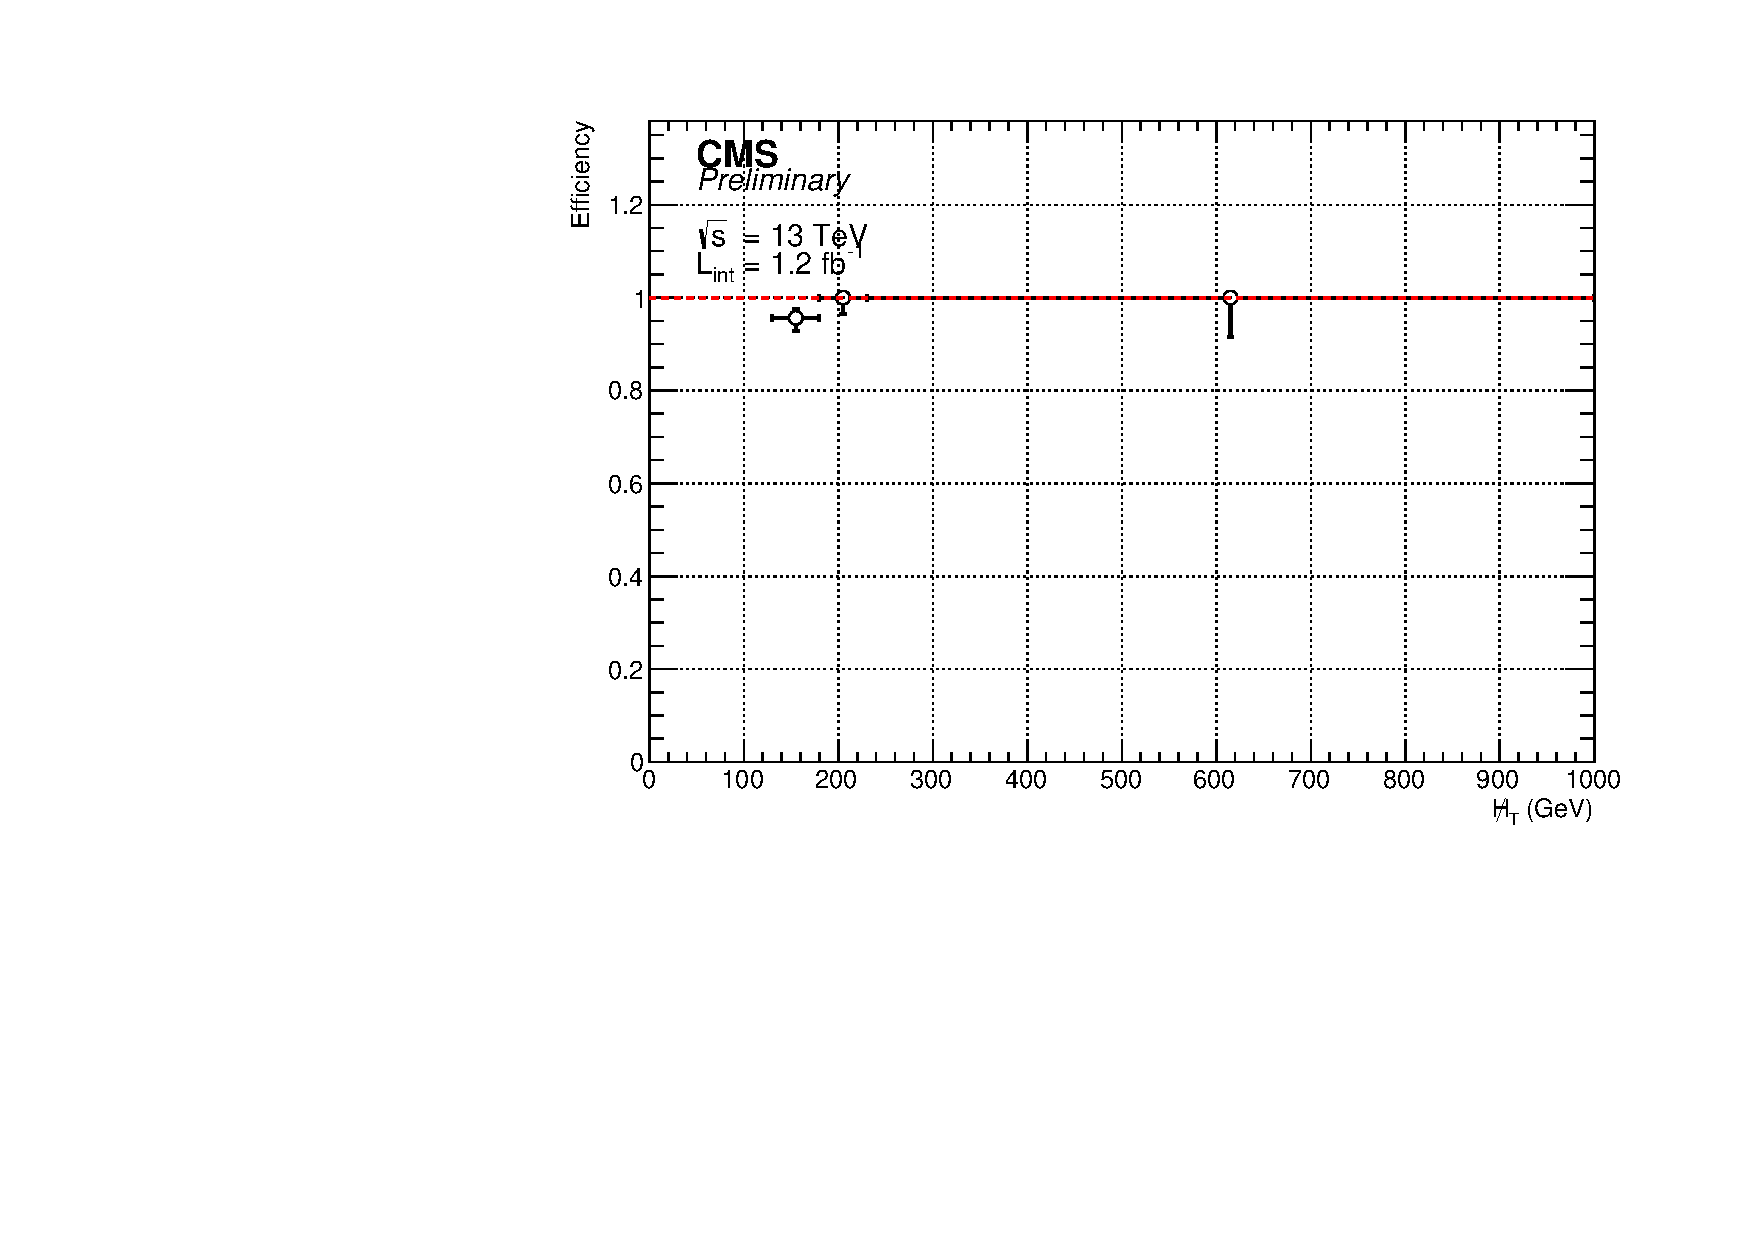
\includegraphics[width=0.5\textwidth]{figures/Trigger/HLT_Ele23_eta2p1_WPLoose_Gsf/HLT_AlphaTMonoAll_MoM_300to350_mht}} ~~\
    \subfigure[$350 < \scalht < 400$]{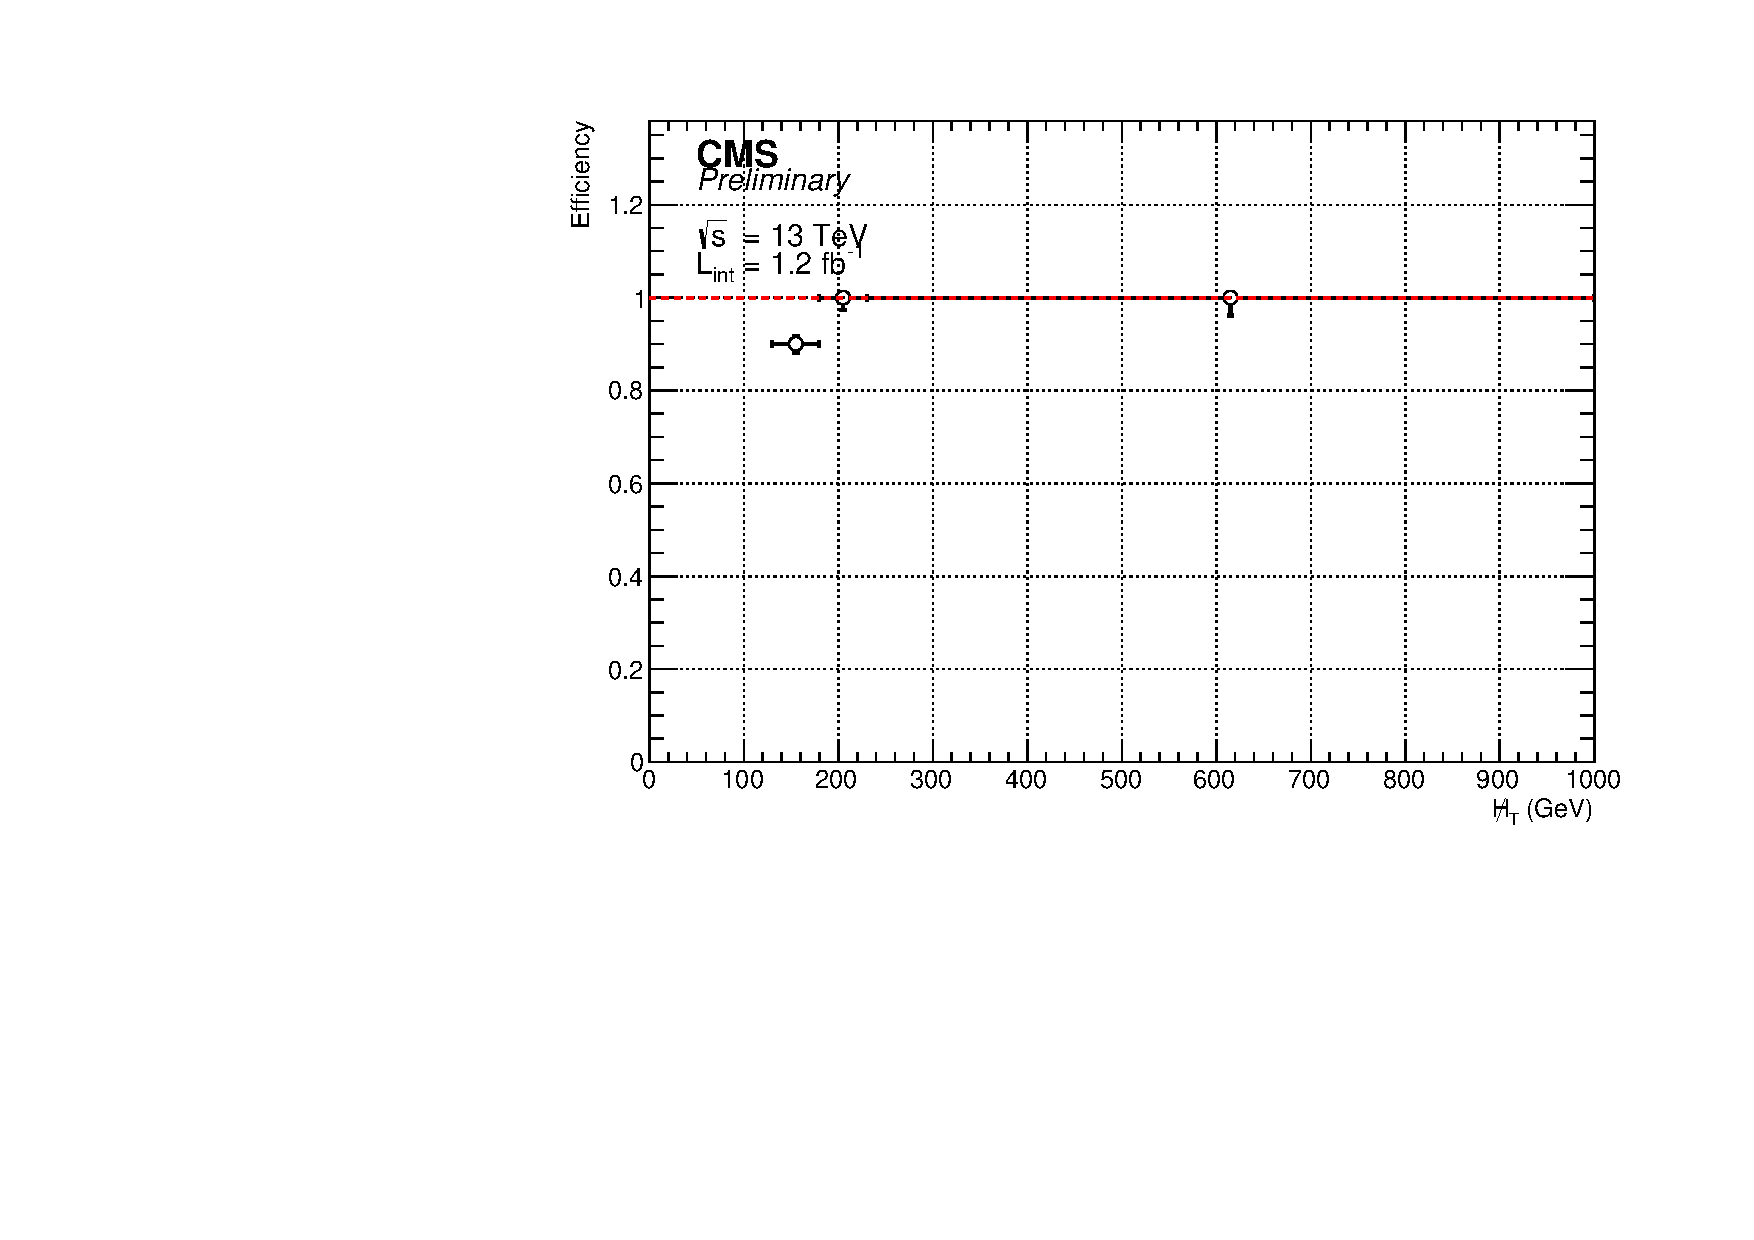
\includegraphics[width=0.5\textwidth]{figures/Trigger/HLT_Ele23_eta2p1_WPLoose_Gsf/HLT_AlphaTMonoAll_MoM_350to400_mht}} \\
    \subfigure[$400 < \scalht < 600$]{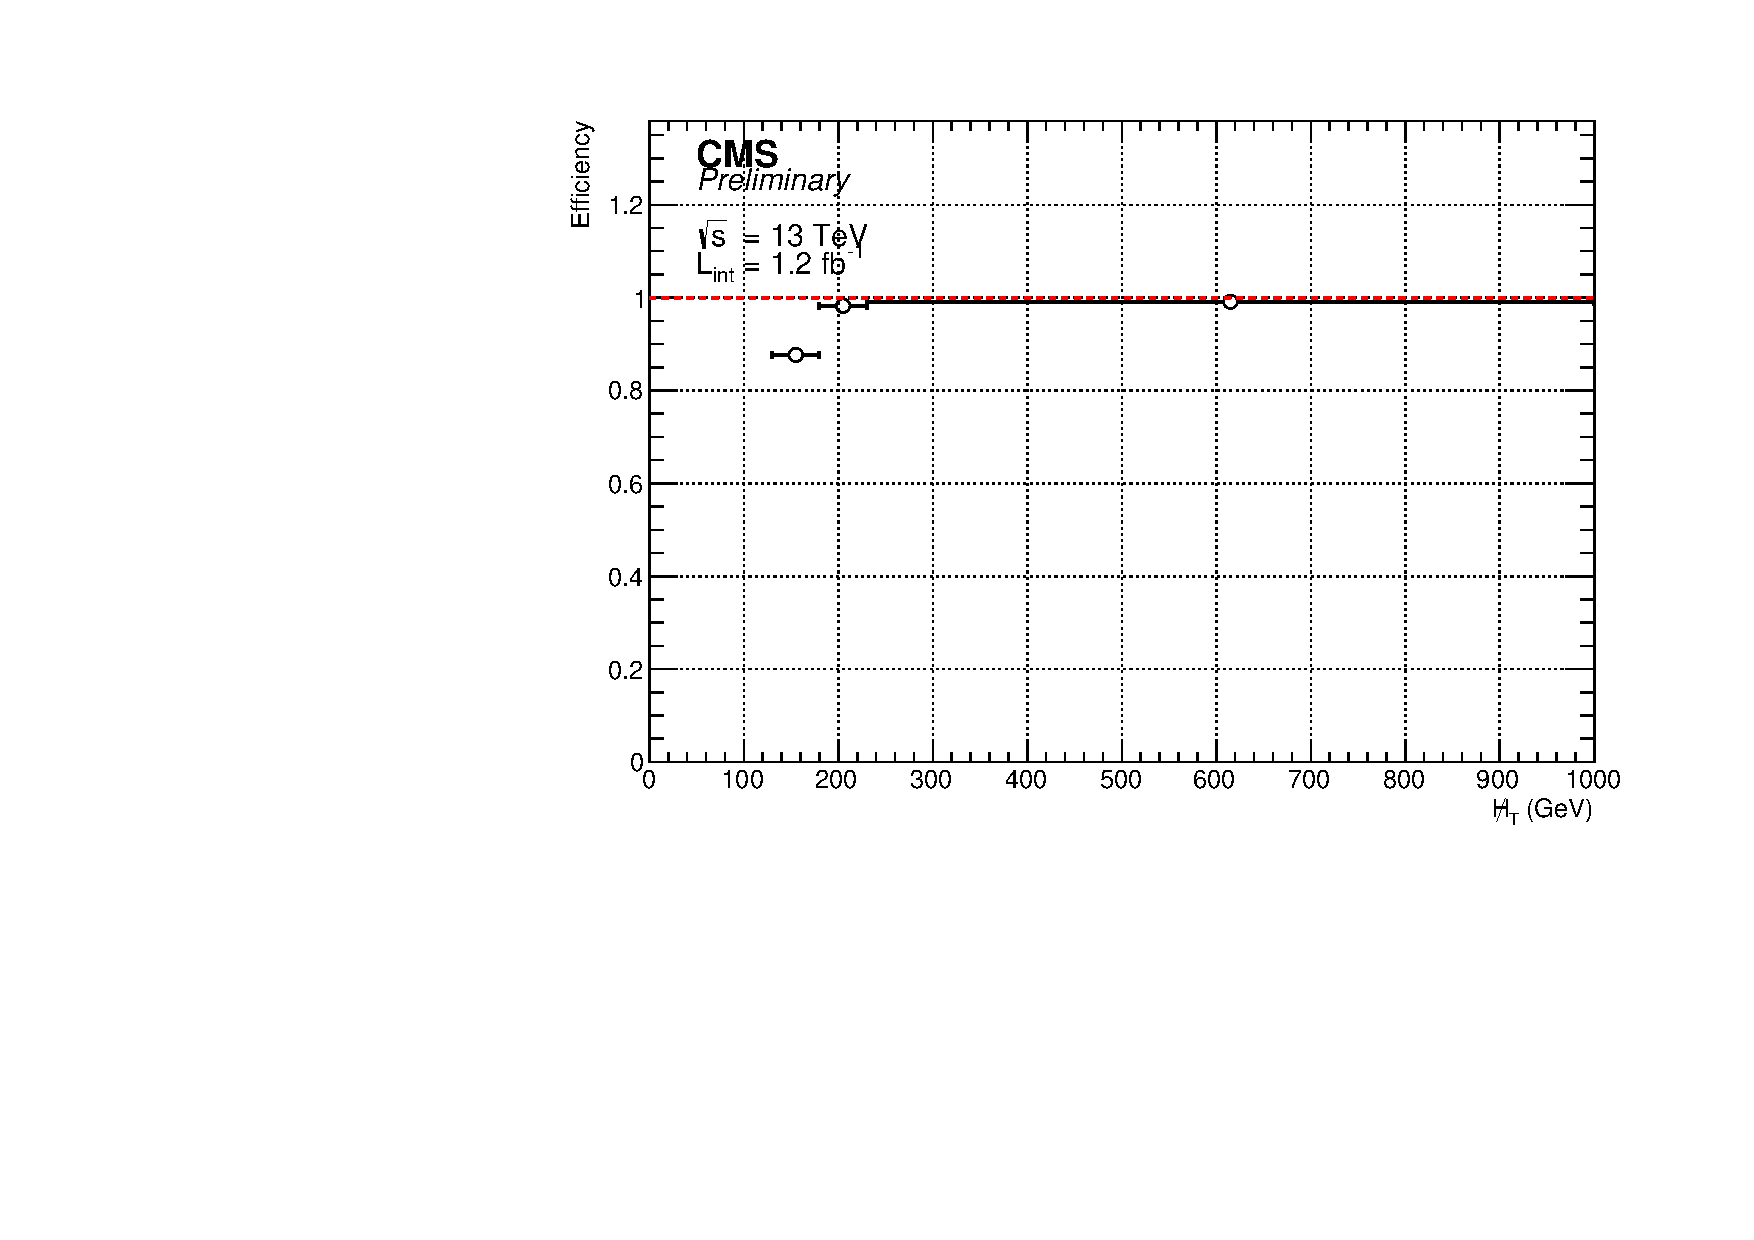
\includegraphics[width=0.5\textwidth]{figures/Trigger/HLT_Ele23_eta2p1_WPLoose_Gsf/HLT_AlphaTMonoAll_MoM_400to600_mht}} ~~\
    \subfigure[$600 < \scalht < 800$]{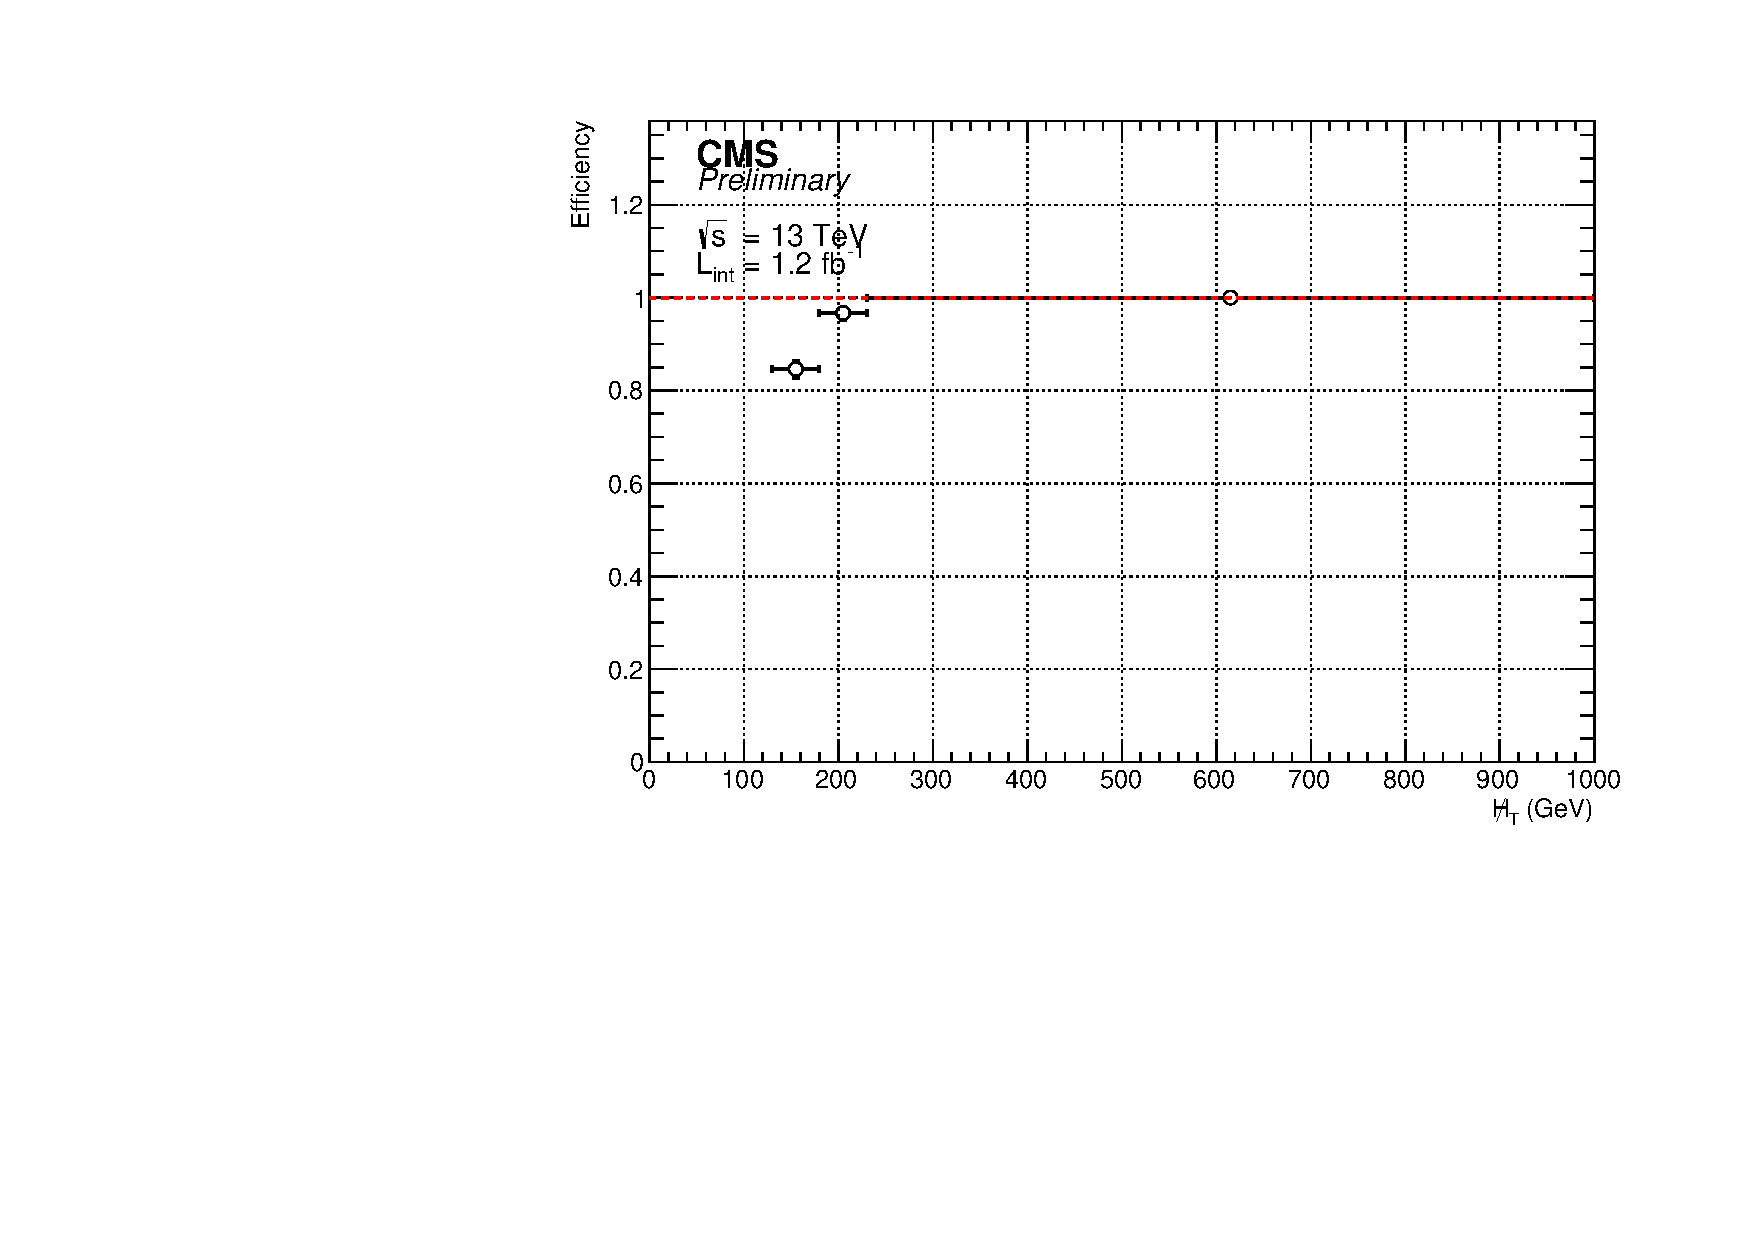
\includegraphics[width=0.5\textwidth]{figures/Trigger/HLT_Ele23_eta2p1_WPLoose_Gsf/HLT_AlphaTMonoAll_MoM_600to800_mht}} \\
    \caption{ Multijet
          }
    \label{fig:alphat_turnons}
  \end{center} 
\end{figure}


\begin{figure}[h!]
  \begin{center}
    \subfigure[$800 < \scalht < 850$]{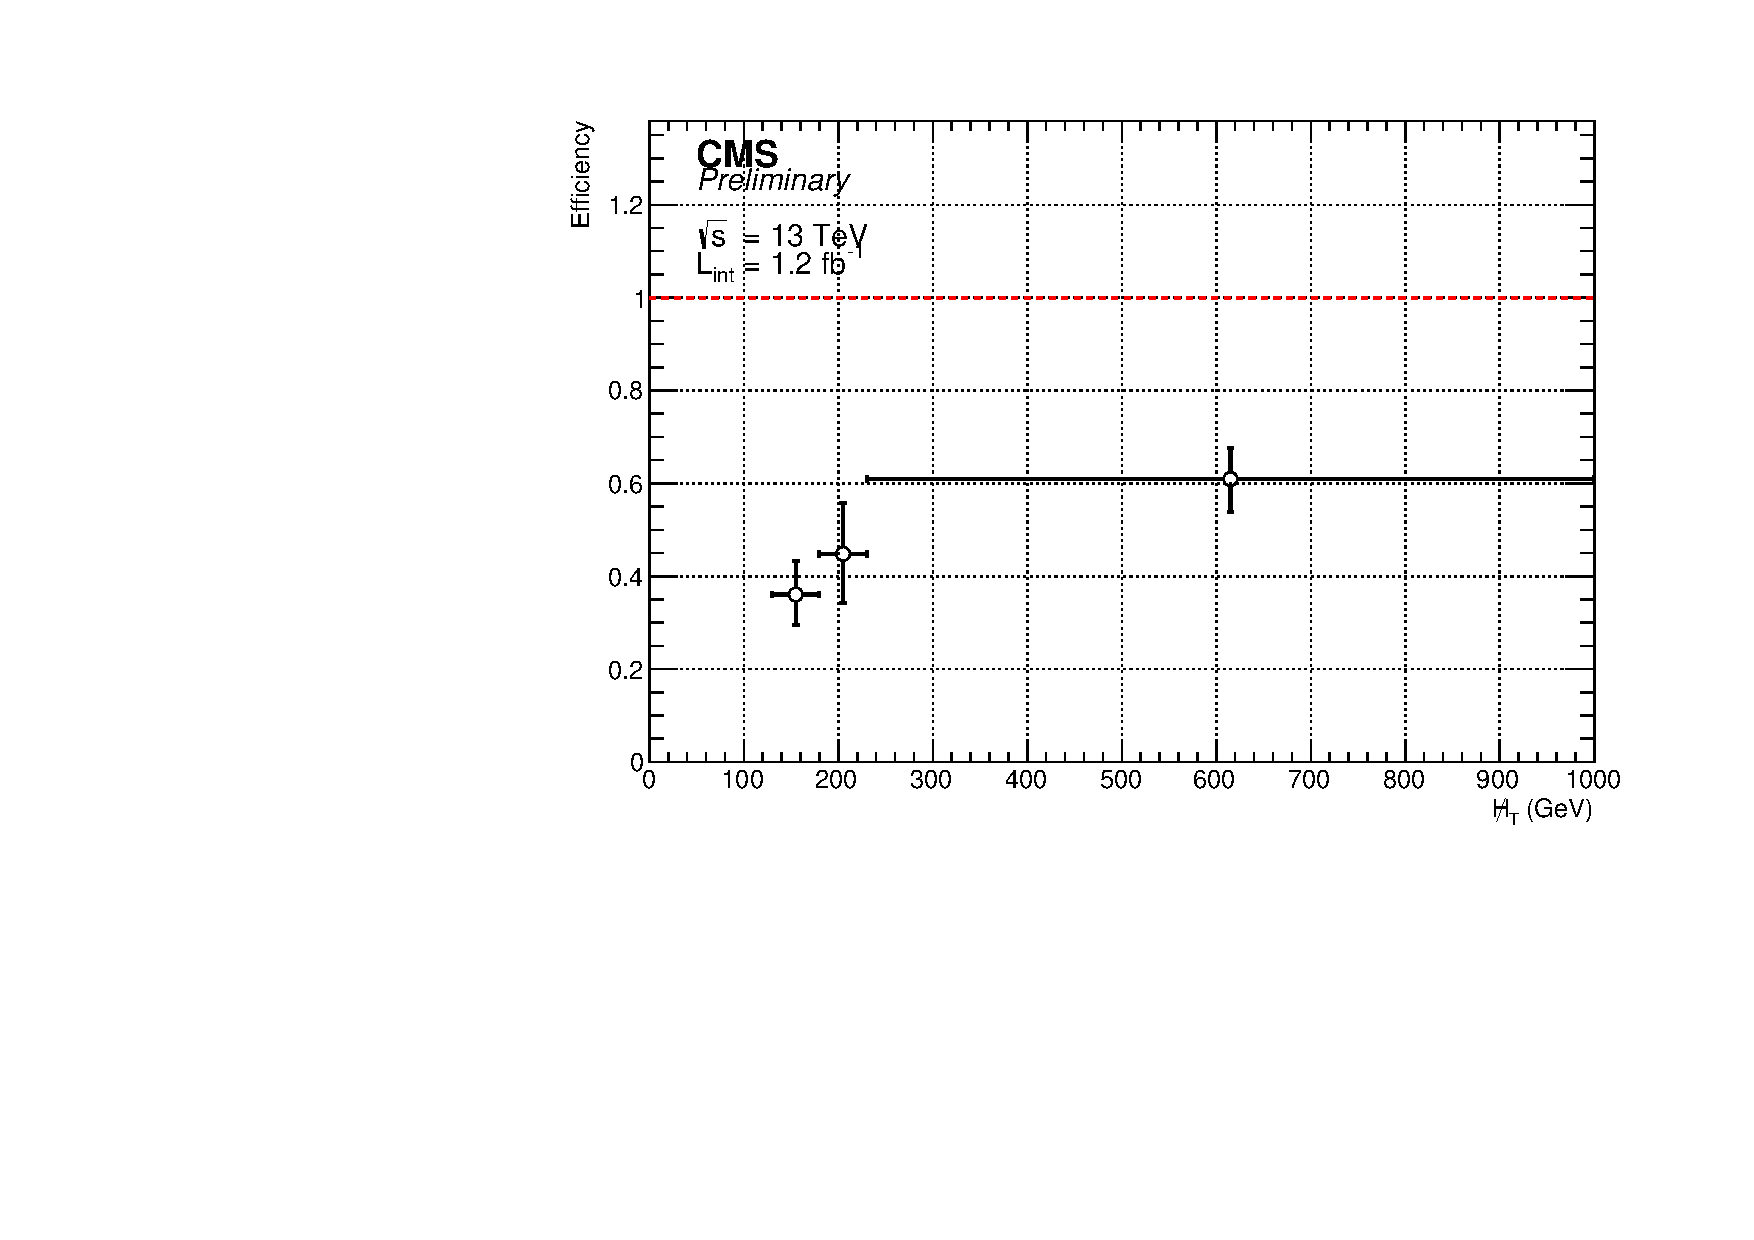
\includegraphics[width=0.5\textwidth]{figures/Trigger/HLT_Ele23_eta2p1_WPLoose_Gsf/HLT_HT800AlphaTAll_MoM_800to850_mht}} ~~\
    \subfigure[$850 < \scalht < 900$]{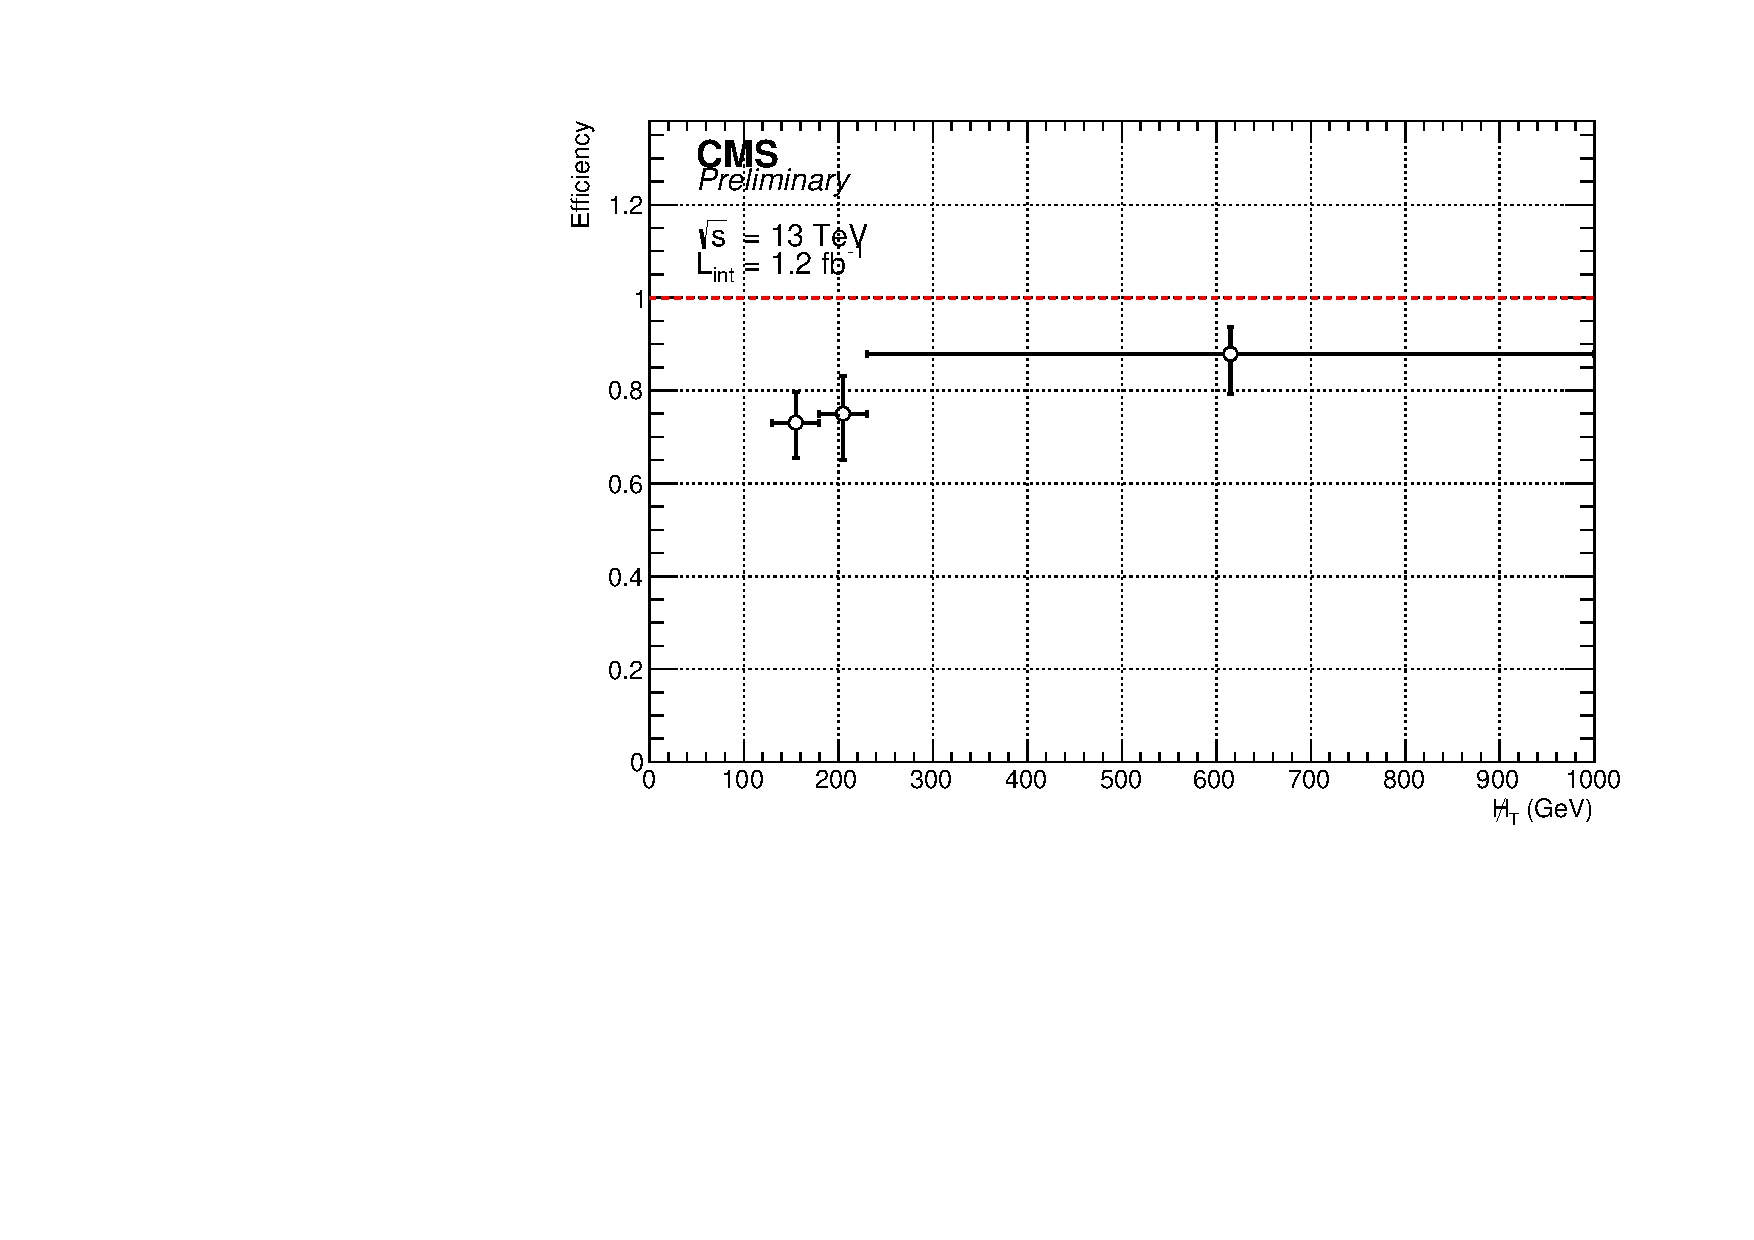
\includegraphics[width=0.5\textwidth]{figures/Trigger/HLT_Ele23_eta2p1_WPLoose_Gsf/HLT_HT800AlphaTAll_MoM_850to900_mht}} \\
    \subfigure[$\scalht > 900$]{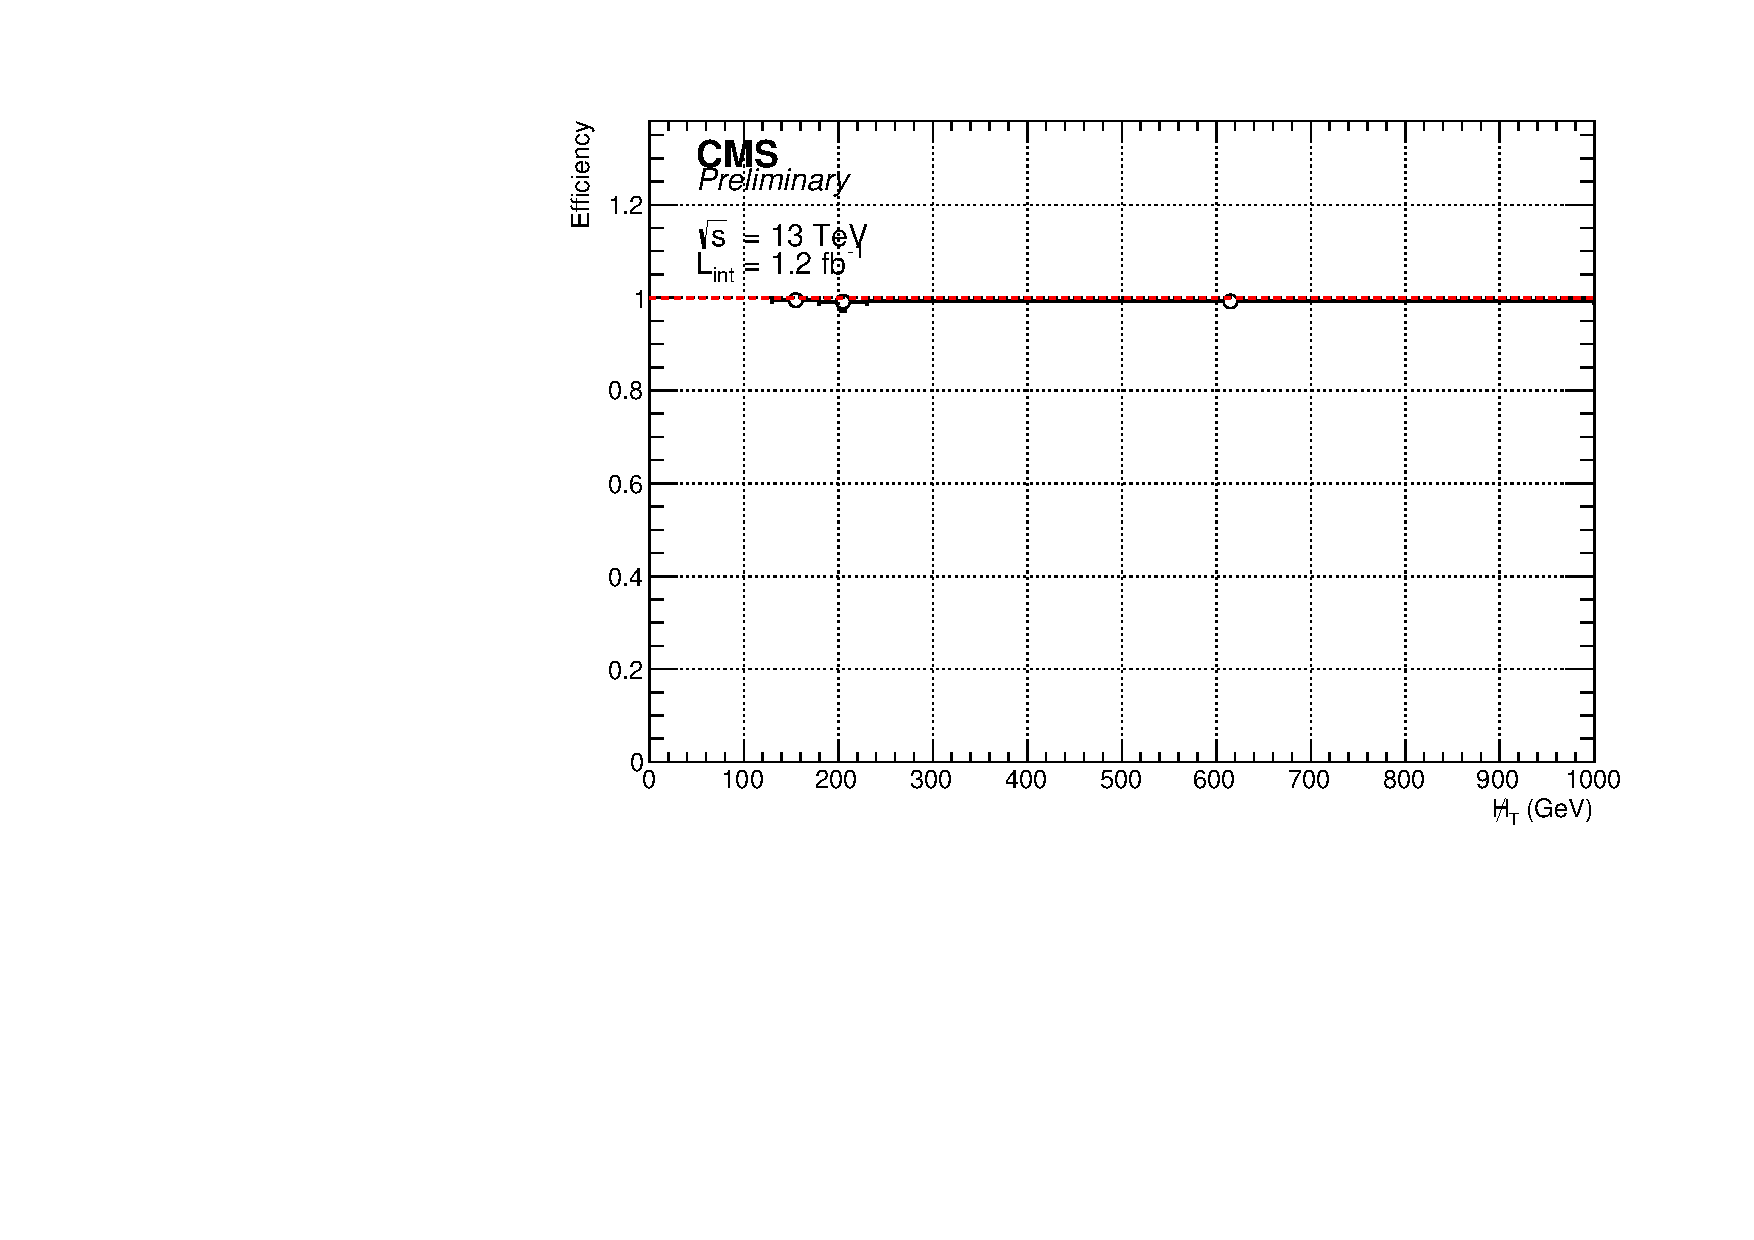
\includegraphics[width=0.5\textwidth]{figures/Trigger/HLT_Ele23_eta2p1_WPLoose_Gsf/HLT_HT800AlphaTAll_MoM_900to999999_mht}} ~~ \\
    \caption{ Multijet
          }
    \label{fig:alphat_turnons}
  \end{center} 
\end{figure}







% Control region triggers
\subsection{Control samples\label{sec:control_samples}}
Prescaled $\scalht$ triggers, \verb!HLT_PFHTXXX!, and a prescaled 
$\scalht$-$\alphat$ cross-trigger, are utilised in the 
selection of events for the hadronic control region. Shown 
in Table~\ref{tab:2015_Hadronic_Control_Triggers} these triggers share the same Level-1 
seeds and $\scalht$ threshold of the signal cross-triggers and are similarly each mapped 
to a unique offline bin. The efficiency of these triggers are similarly measured from an electron 
reference trigger in addition to an independent measurement with the \verb!HLT_Physics! 
minimum bias trigger.


% TABLE: Hadronic control region
%----------------------------------------------------------------------
\begin{table}[h!]
\topcaption{Hadronic control triggers. }
\footnotesize
\centering
\begin{tabular}{c|cc} 
\hline
\hline
HLT path & \multicolumn{1}{c}{Prescale} \\
\hline
\texttt{HLT\_PFHT200} & 3060 \\
\texttt{HLT\_PFHT250} & 2040 \\
\texttt{HLT\_PFHT300} & 1020 \\
\texttt{HLT\_PFHT350} & 180  \\
\texttt{HLT\_PFHT400} & 120  \\
\texttt{HLT\_PFHT200\_PFAlphaT0p51} & 175 \\
\hline
\hline

\end{tabular}
\label{tab:2015_Hadronic_Control_Triggers}
\end{table}


The non-hadronic control regions are seeded by the lowest-threshold unprescaled 
triggers available in the given run scenario. In the high-luminosity scenario The 
\mj and \mmj control samples are selected with the \verb!HLT_IsoMu20! trigger,
and the \gj control sample by the \verb!HLT_Photon175! trigger. 
%The \ej and \eej control samples may be seeded by the \verb!HLT_Ele23_eta2p1_WPLoose_Gsf! trigger.

The efficiency of the control triggers is measured with data-driven methods
(provided by the relevant POG). The tag and probe method is used in the measurement of
efficiencies of the muon and electron triggers and a loose photon reference trigger 
is utilised in the measurement of the photon trigger efficiency. For the results in 
this note for the muon control regions the emulated trigger bit in MC is used to simulate 
the trigger. An offline \Pt requirement of 200\GeV is made on the photon
to ensure it is in the efficiency plateau of the trigger.



%%____________________________________________________________________________||
